\documentclass[
	% -- opções da classe memoir --
%	article,			% indica que é um artigo acadêmico
	11pt,				% tamanho da fonte
	openright,
	twoside,			% Oposto a oneside
	a4paper,			% tamanho do papel. 
	english,			% idioma adicional para hifenização
	french,
	brazil,				% o último idioma é o principal do documento
	sumario=tradicional
	]{abntex2}

\usepackage{lmodern}			% Usa a fonte Latin Modern
\usepackage[T1]{fontenc}		% Selecao de codigos de fonte.
\usepackage[utf8]{inputenc}		% Codificacao do documento (conversão automática dos acentos)
\usepackage{indentfirst}		% Indenta o primeiro parágrafo de cada seção.
\usepackage{nomencl} 			% Lista de simbolos
\usepackage{color}				% Controle das cores
\usepackage{graphicx}			% Inclusão de gráficos
\usepackage{microtype} 			% para melhorias de justificação
% Tabelas longas -> + de uma página
\usepackage{longtable}

\usepackage[brazilian,hyperpageref]{backref}	% Paginas com as citações na bibl
\usepackage[alf]{abntex2cite}					% Citações padrão ABNT

\renewcommand{\backrefpagesname}{Citado na(s) página(s):~}
\renewcommand{\backref}{}
\renewcommand*{\backrefalt}[4]{
	\ifcase #1 %
		Nenhuma citação no texto.%
	\or
		Citado na página #2.%
	\else
		Citado #1 vezes nas páginas #2.%
	\fi}%
% ---

\titulo{Apostila com uma rápida introdução ao SCRUM}
\autor{Paulino Ng\thanks{PANG CO.\\paulino.ng@gmail.com}
}
\local{Brasil}
\data{2019, v-0.5.1}

% informações do PDF
\makeatletter
%\hypersetup{
%     	%pagebackref=true,
%		pdftitle={\@title}, 
%		pdfauthor={\@author},
%    	pdfsubject={Apostila de conceitos básicos de OO},
%	    pdfcreator={PDFLaTeX with abnTeX2 on texmaker},
%		pdfkeywords={OO}{Scott Ambler}{UML}{Java EE}, 
%		colorlinks=true,       		% false: boxed links; true: colored links
%    	linkcolor=blue,         	% color of internal links
%    	citecolor=blue,        		% color of links to bibliography
%    	filecolor=magenta,      	% color of file links
%		urlcolor=blue,
%		bookmarksdepth=4
%}
\makeatother
% --- 

\makeindex

% Altera as margens padrões
% ---
\setlrmarginsandblock{2cm}{2cm}{*}
\setulmarginsandblock{2cm}{2cm}{*}
\checkandfixthelayout

% O tamanho do parágrafo é dado por:
\setlength{\parindent}{1.0cm}

% Controle do espaçamento entre um parágrafo e outro:
\setlength{\parskip}{0.2cm}  % tente também \onelineskip

% Espaçamento simples
\SingleSpacing

\begin{document}
\selectlanguage{brazil}

% Retira espaço extra obsoleto entre as frases.
\frenchspacing 

%\maketitle

\imprimircapa

\pdfbookmark[0]{\contentsname}{lof}
\listoffigures*
%\cleardoublepage*
\newpage 

%\pdfbookmark[0]{\contentsname}{lot}
%\listoftables*
%%\cleardoublepage*
%\newpage

\pdfbookmark[0]{\contentsname}{toc}
\tableofcontents*
%\cleardoublepage*
\newpage 

% resumo em português
\begin{resumoumacoluna}
Este texto objetiva introduzir a metodologia de desenvolvimento SCRUM.

\vspace{\onelineskip}
\noindent
\textbf{Palavras-chave}: SCRUM. Metodologia de Desenvolvimento. Metodologia Ágil.
\end{resumoumacoluna}

\textual

% try to generate a table of contents after summary
%\tableofcontents

\chapter{Rápida introdução ao SCRUM}
%\section{Introdução}
%\addcontentsline{toc}{section}{Introdução}

\section{O Que É Scrum?}
Scrum é um framework projetado para ajudar pequenas equipes unidas a desenvolver produtos complexos. Resultado do trabalho de um punhado de engenheiros de software trabalhando juntos no final do século XX, scrum ganhou força no setor tecnológico, mas não é necessariamente técnico e pode ser facilmente adaptado para outras indústrias. Os autores \citeonline{scrum:brief} dizem que você pode adaptá-lo para construir uma ratoeira melhor, ou para administrar a divisão de \textit{marketing} de uma companhia de cachorrinhos de estimação, ou até para escrever um livro, como eles fizeram.

Uma equipe scrum consiste, tipicamente, de cinco a nove pessoas que trabalham juntas em curtos intervalos de intensa atividade chamadas de arrancadas (\emph{sprints}), com bastante tempo embutido para revisão e reflexão. Um dos mantras de scrum é ``inspecionar e adaptar'' e equipes scrum são caracterizadas por um foco intenso  na melhoria contínua do processo delas e do produto. Nesta seção veremos uma introdução muito rápida da terminologia do scrum: os vários papéis, artefatos e eventos que ocorrem num ciclo de arrancada (\emph{sprint cycle}).

\section{Papéis}
O Scrum conhece três papéis distintos para os membros da equipe:
\begin{description}
\item[Proprietário do Produto] O proprietário do produto (\emph{product owner}) é responsável pela maximização do retorno que o negócio traz ao investimento (ROI - Return-Of-Investment). Ele é o único que controla a ordem, a prioridade, da lista de pendências (\textit{backlog itens}) da equipe. Ele garante que a equipe entende totalmente os requisitos. Ele registra os requisitos na forma de estórias de usuário (\emph{user stories}), por exemplo: ``Como um <papel - tipo de usuário>, quero <uma característica>, de modo que possa <fazer algo>'' e coloca-as na lista de pendências. Cada uma destas estórias de usuário, quando completada, aumentará o valor do produto.

\item[Mestre Scrum] O Mestre Scrum age como um \textit{coach} (treinador), guiando a equipe para níveis mais altos de coesão, auto-organização e desempenho. Enquanto a equipe entrega o produto, o Mestre Scrum entrega uma equipe de alto desempenho e auto-organizada. O Mestre Scrum ajuda a equipe a aprender e aplicar scrum e outras práticas ágeis relacionadas. O mestre scrum está sempre disponível para ajudar a equipe na remoção de obstáculos que estejam bloqueando a execução do trabalho. O mestre scrum não é o chefe, ele é um membro da equipe que se destaca pelo seu conhecimento e suas responsabilidades.

\item[Membro de Equipe] Equipes scrum de alto desempenho são altamente colaborativas, elas também são auto-organizadas. Os membros da equipe têm total autoridade sobre como o trabalho é realizado. A equipe decide por si quais são as ferramentas a serem usadas e quais membros irão trabalhar em quais tarefas. Se o negócio precisa de estimativas de cronograma, são os membros da equipe que criam as estimativas. Uma equipe scrum deve possuir todas as capacitações necessárias para criar um produto entregável. Ocasionalmente, pode ser que um membro tenha de trabalhar fora da sua especialidade para que um item da lista de pendências (uma estória de usuário) saia do estado ``progredindo'' para ``feito''. Esta é uma mudança de mentalidade do ``faço meu serviço'' para ``faço o serviço''. 

\end{description}

O proprietário do produto:
\begin{itemize}
\item detém a visão do produto;
\item representa os interesses do negócio;
\item representa os clientes (\textit{stockholders});
\item é dono da lista de pendências do produto (\textit{product backlog});
\item ordena, prioriza, os itens da lista de pendências do produto;
\item cria critérios de aceitação para os itens da lista de pendências do produto; e
\item está disponível para responder às dúvidas dos outros membros da equipe.
\end{itemize}

O papel do Mestre Scrum é ser:
\begin{itemize}
\item especialista e orientador de scrum;
\item treinador;
\item quebrador de barreiras; e
\item facilitador.
\end{itemize}

O papel de Membro da Equipe:
\begin{itemize}
\item é ser responsável por completar as estórias do usuário para incrementar o valor do produto;
\item se auto-organizar para conseguir que todo o trabalho necessário seja feito;
\item criar suas próprias estimativas de cronogramas;
\item decidir ``como fazer o trabalho''; e
\item fugir do pensamento ``não é meu serviço''.
\end{itemize}

\section{Artefatos do Scrum}
\subsection{A Lista de Pendências do Produto (\emph{Product Backlog})}
A lista de pendências do produto é uma lista acumulativa de itens entregáveis desejados para o produto. Isto inclui características, consertos de erros (\emph{bug fixes}), alterações na documentação e qualquer outra coisa que seja significativa e valiosa para produzir. Embora pendência seja um termo correto para um item da lista, as equipes de scrum preferem usar o termo estória de usuário para reforçar a noção de que construímos produtos para satisfazer as necessidades dos usuários.

Cada item da lista deve incluir as seguintes informações:
\begin{itemize}
\item Quais usuários vão se beneficiar da estória;
\item Uma rápida descrição da funcionalidade desejada (o que precisa ser construído);
\item A razão para a estória ser preciosa (por que precisamos realizá-la);
\item Uma estimativa de quanto trabalho será necessário para realizar a estória; e
\item Critérios de aceitação que ajudarão a saber se a implementação está correta.
\end{itemize}

\subsection{A Lista de Pendências da Arrancada (\emph{Sprint Backlog})}
A lista de pendências da arrancada é a lista de coisas a fazer na arrancada, período fixo de tempo de trabalho. Diferente da lista de pendências do produto, ela tem tempo de vida finito: a duração da arrancada. Ela inclui todas as estórias e tarefas associadas que a equipe se compromete a realizar nesta arrancada. Estórias são entregas e podem ser pensadas como unidades de valor. Tarefas são coisas que precisam ser feitas, para entregar as estórias, logo, tarefas podem ser vistas como unidades de trabalho. Uma estória é algo que uma equipe entrega; Uma tarefa é um pedaço de trabalho que alguém faz. Cada estória normalmente requer muitas tarefas.

\subsection{Gráficos de Queimada}
Um gráfico de queimada (\emph{burn chart}) nos mostra a relação entre o tempo e o escopo. O tempo está no eixo horizontal X e o escopo está no eixo vertical Y. Um gráfico de queimada nos mostra quanto de escopo uma equipe conseguiu realizar num período de tempo. Cada vez que algo é completado, a linha no gráfico se move para cima. Um gráfico de queimada nos mostra o que falta fazer. Em geral, esperamos que o trabalho restante diminua com o tempo à medida que a equipe termina tarefas. Às vezes, o trabalho restante muda de repente, quando escopo é adicionado ou retirado. Estes eventos aparecem como linhas verticais no gráfico de queimada.

\subsection{Quadro de Tarefas}
Para todos os integrantes da equipe Scrum acompanharem o andamento do trabalho, um quadro de tarefas é colocado numa sala usada por todos os integrantes. Isto evita que alguma parte importante do trabalho seja esquecida.

O quadro de tarefas mais simples tem três colunas: A fazer, Fazendo e Terminada. As tarefas são deslocadas através das colunas do quadro, fornecendo visibilidade para quais tarefas foram terminadas, quais estão sendo feitas e quais ainda não começaram. Esta visibilidade ajuda a equipe a ver a situação atual e se adaptar conforme a necessidade. O quadro também ajuda os clientes a verem o progresso que a equipe está fazendo. Com a ideia de usar os artefatos mais simples, o quadro é uma superfície onde podemos colar \textit{post-it}s com as tarefas escritas neles. Estes post-its são colocados nas 3 colunas conforme a evolução das atividades.

\begin{center}
\parbox{16cm}{
\textbf{Definição de Terminada}\\
\textit{Terminada} é uma palavra fantástica, quando a equipe consegue que uma estória de usuário seja terminada, é hora de festejar. Mas, às vezes, há uma certa confusão sobre o que exatamente \emph{terminada} significa. Um programador pode dizer que alguma coisa está terminada quando o código está escrito. Um testador pode pensar que terminada significa que todos os testes passaram. O pessoal de operações pode pensar que terminada significa que os programas foram carregados nos servidores de produção. Uma pessoa do comercial pode pensar que terminada significa que podemos vender aos clientes e que está pronta para uso. Esta confusão sobre o que \emph{terminada} significa pode causar problemas, quando, por exemplo, o vendedor pergunta por que a equipe ainda está trabalhando numa estória que o programador disse estar terminada há duas semanas.

Para evitar confusão, as boas equipes de scrum devem ter sua definição de como a palavra \emph{terminado} se aplica a uma estória de usuário. Elas decidem juntas que coisas precisam ser concluídas antes da equipe declarar que uma estória foi terminada. A definição da equipe pode incluir coisas como: código escrito, código revisto, aprovação nos testes unitários, documentação escrita, assinatura do proprietário do produto, ... Esta é a lista de coisas, que a equipe concorda em fazer sempre antes de declarar que uma estória está terminada, é a definição da equipe do que significada estória \emph{terminada}. A equipe deve imprimir a definição de terminada como uma lista a ser checada próxima do quadro de tarefas. Quando a equipe acha que uma \emph{estória} está \emph{terminada}, verifica-se que todos os itens da lista foram concluídos.
}

\end{center}

\section{O Ciclo da Arrancada (\textit{Sprint Cycle})}

O ciclo da arrancada consiste de várias reuniões, chamadas de cerimônias, para satisfazer as pessoas que não gostam da palavra reunião:
\begin{itemize}
\item planejamento da arrancada;
\item scrum diário;
\item hora da estória;
\item revisão da arrancada e
\item retrospectiva.
\end{itemize}

\noindent \textbf{É uma questão de ritmo}

O ciclo da arrancada é o ritmo fundamental do processo scrum. Como quer que você chame seu período de desenvolvimento: Uma arrancada (\emph{sprint}), um ciclo, ou uma iteração. Você está sempre falando da mesma coisa: Um \emph{período fixo} de tempo no qual você mastiga pedaços do seu projeto e termina-os antes de morder mais. No final da arrancada, você mostrará algum software funcionando.

Quanto mais frequente forem as entregas da equipe de incrementos do produto, maior a liberdade do negócio para decidir quando e o que entregar. Observe que existem duas decisões separadas a serem tomadas aqui:

\begin{description}
\item[O produto tem potencial para ser comercializado?] Isto é, a qualidade é boa o suficiente para que seja comercializado? Todas as estórias atuais terminaram? Esta é uma decisão da equipe.
\item[Tem sentido comercializar o que temos no momento?] Existe valor agregado suficiente para levar o produto atual para o mercado? Esta é uma decisão de negócios.
\end{description}

Adicionalmente, quanto maior a frequência com que a equipe produz incrementos entregáveis do produto, maior a frequência de retornos para a equipe, o que alimenta o importante ciclo de inspecionar-e-adaptar. Quanto mais curto o ciclo da arrancada, com maior frequência a equipe produz valor para o negócio.

Por volta do inicío dos anos 2010, as equipes de scrum trabalhavam com arrancadas de duas semanas e muitas equipes começavam a trabalhar com arrancadas de uma semana. Muitos dos escritos originais de scrum assumiam arrancadas com um duração de um mês e naquela época, isto parecia curto.

A tabela da figura \ref{fig:sprint} esboça o mapeamento das cerimônias que você deve agendar para uma arrancada de uma semana. A duração das cerimônias são uma sugestão inicial, as equipes devem adaptar para suas próprias características.

\begin{figure}[h]
\begin{center}
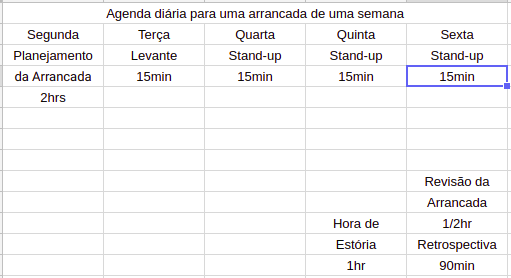
\includegraphics[scale=0.6]{sprint_planning.png}
\caption{Agenda diária para um Sprint de uma semana} \label{fig:sprint}
%\legend{Fonte: \citeonline{wiki:RUP}}
\end{center}
\end{figure}

\subsection{Cerimônia de Planejamento da Arrancada}

A cerimônia de planejamento da arrancada marca o início da arrancada. O objetivo da primeira parte da cerimônia é o comprometimento da equipe para a entrega dos produtos da arrancada. Na segunda parte da cerimômia, a equipe identifica as tarefas que devem ser completadas para as entregas baseadas nas estórias de usuários. Recomenda-se uma cerimônia de planejamento de uma a duas horaas de duração por semana de desenvolvimento.

\noindent \textbf{\small Parte Um: O que faremos?}

A meta da primeira parte da cerimônia de planejamento da arrancada é ter um conjunto de estórias que a totalidade da equipe se compromete a entregar no fim da arrancada. O \emph{proprietário do produto} lidera esta parte da cerimônia.

Uma a uma, na ordem decrescente de prioridade, o proprietário do produto apresenta as estórias que ele gostaria que a equipe completasse durante a arrancada. A medida que cada estória for apresentada, os membros da equipe a discutem com o proprietário do produto e reveem critérios de aceitação para ter certeza que eles têm um entendimento único do que se espera. Então, os membros da equipe decidem se eles podem se comprometer na entrega da estória no final da arrancada. Este processo se repete para cada estória até que a equipe sinta que não pode mais se comprometer com mais trabalho. Observe a separação de autoridade, o proprietário do produto decide quais são as estórias a serem consideradas, mas são os membros da equipe que realizam o trabalho que decidem quanto trabalho eles podem fazer.

\noindent \textbf{\small Parte Dois: Como faremos?}

Na fase dois da cerimônia de planejamento da arrancada, a equipe começa a decompor as estórias selecionadas em tarefas. Lembre-se que as estórias são os produtos entregáveis: Coisas que os contratantes, usuários e clientes querem. Para entregar uma estória, os membros da equipe terão de terminar as tarefas. Tarefas são coisas como: Obtenha mais entradas dos usuários; projete uma nova tela; adicione colunas a um banco de dados; escreva texto de ajuda (help); Faça a tradução do menu para as localidades alvo; execute os scripts de entrega.

O proprietário do produto deve estar disponível pelo menos durante metade da cerimônia para responder às questões. A equipe pode também precisar ajustar a lista de estórias para a qual ela está se compromentendo, já que na fase de identificação das tarefas, os membros da equipe podem percerber que eles se comprometeram com um excesso de estórias ou com um número insuficiente.

O resultado da cerimônia de planejamento da arrancada é o \textit{sprint backlog} (a lista de pendências da arrancada), a lista de todas as estórias que a equipe se compromete a entregar, com as tarefas associadas. O proprietário do produto concorda em não pedir estórias adicionais durante a arrancada, a menos que a equipe especificamente solicite mais. O proprietário do produto também concorda em está disponível para responder questões sobre as estórias, negociar o escopo delas e fornecer orientações sobre o produto até as estórias serem aceitáveis e forem consideradas terminadas.

\subsection{Scrum Diário}

A cerimônia de scrum diário, chamada às vezes de \textit{stand-up meeting}, é:
\begin{description}
\item[Diária:] A maioria das equipes escolhe fazer esta cerimônia no início do dia de trabalho. Você pode adaptá-la para as preferências da sua equipe.
\item[Breve:] Um ponto desta cerimônia é desencorajar as discursões e os desvios que tornam as reuniões um inferno. O scrum diário deve sempre durar no máximo 15 minutos.
\item[Direta:] Cada participante rapidamente compartilha:
\begin{itemize}
\item Quais tarefas completei desde o último scrum diário;
\item Quais tarefas espero completar até o próximo scrum diário; e
\item Quais obstáculos estão me retardando.
\end{itemize}
\end{description}

O objetivo desta cerimônia é inspecionar e adaptar o trabalho dos membros da equipe para que as estórias comprometidas pela equipe sejam completadas com sucesso. A inspeção acontece na cerimônia, a adaptação pode ser feita depois dela. Isto significa que a equipe não precisa resolver os problemas na cerimônia, apenas trazer à torna as questões e decidir quais membros da equipe vão se ocupar delas é, normalmente, o suficiente. Lembre-se, a cerimônia é breve.

\subsection{Hora de Estória}

Nesta cerimônia, você discutirá e melhorará as estórias na lista de pendências do produto, \emph{product backlog}, que contém todas as estórias para as futuras arrancadas. Observe que não são as estórias da arrancada atual, estas estão nas pendências da arrancada, \emph{sprint backlog}. Recomenda-se que a cerimônia dure uma hora por semana, toda semana, independente da duração da sua arrancada. Nesta cerimônia, a equipe trabalha com o proprietário do produto para:

\noindent \textbf{\small Definir e Redefinir Critérios de Aceitação}

Cada estória de usuário na lista de pendências do produto deve incluir uma lista de critérios de aceitação. Estas são condições testáveis para aprovado/reprovado que nos ajudam a saber quando uma estória está implementada como se pretendia. Algumas pessoas pensam nelas como exemplos de aceitação: Os exemplos que a equipe vai usar para mostrar que uma estória está terminada.

\noindent \textbf{\small Tamanho da Estória}

Durante a cerimônia do tempo de estória, a equipe vai atribuir (ou estimar) um tamanho para as estórias que ainda não tiverem seus tamanhos estimados. O tamanho é uma adivinhação da equipe sobre a quantidade de trabalho que uma estória necessita para ser completada.

\noindent \textbf{\small Divisão da estória}

Estórias no topo da lista de pendências do produto precisam ser pequenas. Estórias pequenas são fáceis para todos entenderem e fáceis para a equipe completar em um curto espaço de tempo. Estórias mais no fundo da lista de pendências do produto podem ser maiores e menos bem definidas. Isto implica em que temos de quebrar estórias maiores em estórias menores a medida que as estórias sobem na lista. Enquanto o proprietário do produto pode fazer esta quebra por conta própria, o tempo de estória é a oportunidade dele ter ajuda de todo a equipe para esta atividade.

A cerimônia do tempo de estória não é uma \emph{cerimônia oficial} do scrum. Mas as equipes de scrum de alto desempenho costumam usá-la.

\subsection{Revisão da Arrancada}

Este é o final público da arrancada, convide todos os interessados (\textit{stockholders}) para esta cerimônia. É a oportunidade da equipe mostrar seus sucessos, as estórias que cumpriram a definição de terminada da equipe. Esta também é uma oportunidade para os interessados verem como o produto melhorou com a arrancada.

Se existirem estórias que a equipe se comprometeu a terminar, mas não conseguiu, este é o momento para compartilhar esta informação com os interessados. O evento principal desta cerimônia é, obviamente, mostrar as estórias terminadas. Sem dúvidas, os interessados darão um retorno e idéias que o proprietário do produto e a equipe usarão na fase de inspeção-e-adaptação do produto.

Esta cerimônia não é uma reunião para tomar decisões. Não é onde decidimos se uma estória está terminada, isto é feito antes. Não é quando decidimos sobre o que faremos em seguida, na próxima arrancada, isto é feito na cerimônia de planejamento da arrancada.
Quão longa deve ser a cerimônia de revisão da arrancada? Recomenda-se que seja agendada por meia hora a uma hora por semana de desenvolmento.

\subsection{Retrospectiva}

Enquanto a revisão da arrancada é o término público da arrancada, a equipe ainda tem mais uma cerimônia: A retrospectiva. Scrum foi projetado para ajudar as equipes a inspecionar e adaptar continuamente, resultando em desempenho cada vez melhor e felicidade. A retrospectiva, que tem lugar no final de cada arrancada, é um tempo dedicado para a equipe se focar no que foi aprendido durante a arrancada e como este aprendizado pode ser usao para melhorar a equipe. Recomenda-se uma a duas horas por semana de desenvolvimento.

Diferente da análise \textit{post mortem}, o objetivo de uma retrospectiva nunca é gerar uma longa lista de lavagem das coisas que funcionaram e das que deram errado, mas identificar uma ou duas mudanças de estratégia para a próxima arrancada. Ela serve para melhorar o processo.

\subsection{Término Anormal da Arrancada}

Em scrum, o acordo básico entre a gerência e a equipe é que a gerência não vai mudar os requisitos durante uma arrancada. Ainda assim, às vezes, algo acontece que invalida tudo no plano de uma arrancada -- o negócio é vendido, uma tecnologia disruptiva entra no mercado, um competidor faz um movimento. A decisão de terminar uma arrancada mais cedo é fundamentalmente uma decisão de negócios, logo o proprietário do produto é quem pede o término anormal de uma arrancada.

Se o proprietário do produto decide terminar precipitadamente uma arrancada, a equipe deve voltar ao estado anterior à arrancada para não trabalhar com modificações incompletas. Realizar uma cerimônia de retrospectiva é particularmente importante após um término anormal para ajudar a equipe a aprender com a experiência.

\subsection{Inspecione e Adapte}

Então, por que desenvolvemos o trabalho em ciclos curtos? Para aprender. Experiência é o melhor professor e o ciclo de scrum é projetado para lhe fornecer várias oportunidades de receber retornos -- dos clientes, da equipe, do mercado -- e aprender com eles.
O que você aprende ao trabalhar num ciclo, prepara você para o planejamento do próximo ciclo. Em scrum, chamamos isto de \emph{inpecionar-e-adaptar}. Você pode chamá-lo de \emph{melhoria contínua}. De qualquer modo, é uma coisa boa.


%\section{Programação J2EE}


% ---
% Finaliza a parte no bookmark do PDF, para que se inicie o bookmark na raiz
% ---
\bookmarksetup{startatroot}% 
% ---

% ---
% Conclusão
% ---
%\section*{Considerações finais}
%\addcontentsline{toc}{section}{Considerações finais}
%
%Texto qualquer.
%
%\begin{citacao}
%Mais texto genérico.
%\end{citacao}
%
%Texto.

% ----------------------------------------------------------
% ELEMENTOS PÓS-TEXTUAIS
% ----------------------------------------------------------
\postextual

% ---
% Título e resumo em língua estrangeira
% ---

% \twocolumn[    		% INICIO DE ARTIGO EM DUAS COLUNAS

% titulo em inglês
%\titulo{Canonical academic article model with \abnTeX}
%\emptythanks
%\maketitle
%
%% resumo em português
%\renewcommand{\resumoname}{Abstract}
%\begin{resumoumacoluna}
% \begin{otherlanguage*}{english}
%   According to ABNT NBR 6022:2003, an abstract in foreign language is a back
%   matter mandatory element.
%
%   \vspace{\onelineskip}
% 
%   \noindent
%   \textbf{Keywords}: latex. abntex.
% \end{otherlanguage*}  
%\end{resumoumacoluna}

% ]  				% FIM DE ARTIGO EM DUAS COLUNAS
% ---

% ----------------------------------------------------------
% Referências bibliográficas
% ----------------------------------------------------------
\bibliography{oo_refs}
\

\end{document}
